\documentclass{svproc}
\usepackage{times}
\usepackage{format}
\usepackage{macros}
\usepackage{macros_stm}
\usepackage{paper}
\usepackage{url}
\usepackage[colorlinks=true,linkcolor=blue,urlcolor=blue,citecolor=blue]{hyperref}
\begin{document}

\newboolean{showcomments}
\setboolean{showcomments}{true}
\ifthenelse{\boolean{showcomments}}
{ \newcommand{\mynote}[3]{
   \fbox{\bfseries\sffamily\scriptsize#1}
   {\small$\blacktriangleright$\textsf{\emph{\color{#3}{#2}}}$\blacktriangleleft$}}}
{ \newcommand{\mynote}[3]{}}
% One command per author:
\newcommand{\pf}[1]{\mynote{Pierre}{#1}{red}}
\newcommand{\hm}[1]{\mynote{Patrick}{#1}{pink}}
\newcommand{\vs}[1]{\mynote{Valerio}{#1}{blue}}
\newcommand{\ft}[1]{\mynote{Francois}{#1}{green}}

\newcommand{\sser}{\textsc{S+Ser}\xspace}
\newcommand{\opa}{\textsc{Opa}\xspace}
% tentative results 
% https://docs.google.com/spreadsheets/d/1jqpC7ehu48kJc96EYcEFRbjgV9wq8E9HbdZpwREfw7w/edit#gid=1043149494
% slides from euro-tm 2014
% https://docs.google.com/presentation/d/1AFntDVRBWmjOMjNzX90ZGo0cG4Jd7Pewas4CeemD5TQ/edit#slide=id.p

\author{(authors omitted due to double-blind review policy)}

\title{A Locality-Aware Software Transactional Memory}

\maketitle

\begin{abstract}
  Software transactional memory (STM) guarantees that a sequence of operations encapsulated into a transaction is atomic.
  This simple yet powerful paradigm is a promising direction for writing concurrent applications.
  %
  Recent STM designs employ a time-based approach to leverage the performance advantage of invisible reads.
  With the advent of many-core architectures and non-uniform memory architecture (NUMA),
  this design is however hitting the synchronization wall of the cache coherency protocol.
  %
  In this paper, we propose a novel and flexible approach to address this limitation.
  Our idea is to leverage the parallelism and the locality of applicative workloads to execute few global operations.
  To that end, we introduce a new STM design that supports invisible reads, lazy snapshots 
  and can be tailored to be either disjoint access parallel, or NUMA-aware.
  Several empirical comparisons against a well-established STM design demonstrate that our design greatly improve perfmance\vs{check it matchs eval content}.
\end{abstract}

\section{Introduction}
\labsection{introduction}

% why TM
The advent of chip level multiprocessing in commodity hardware has pushed applications to be more and more parallel in order to leverage the increase of computational power.
However, the art of concurrent programming is known to be a difficult task~\cite{Lee:2006:PT:1137232.1137289}, and new paradigms are required to help the programmer.
Among those paradigms, transactional memory (TM) is widely considered as a promising direction, in particular thanks to its simplicity~\cite{Dragojevic:2011:WSM:1924421.1924440}.

% the case for invisible optimistic reads and DAP
The engine that orchestrates concurrent transactions run by the application, i.e., the concurrency manager, is one of the core aspects of a STM implementation.
A large number of concurrency manager implementations exists, ranging from pessimistic lock-based implementations\vs{ref?} to completely optimistic ones\vs{ref?}, with~\cite{perelman2011smv} or without multi-version support\vs{ref?}.
Because application workloads exhibit in general a high degree of parallelism\vs{is this a known fact? for which applications? a ref that assess this statement would be good imho}, these designs tend to favor optimistic concurrency control.
In particular, a widely accepted approach consists in executing tentatively invisible read operations and validating them on the course of the transaction execution to enforce consistency.
Another property of interest is disjoint-access parallelism (DAP) \cite{}.
DAP ensures that concurrent transactions operating on disjoint part of the application do not contend in the concurrency manager.
This property is key to ensures that the system scales with the numbers of cores.

% why OPA
From a developper point of view, the interleaving of transactions must satisfy some form of correctness.
Strict serializability (SSER) is a consistency criteria commonly encountered in database litterature.
This criteria ensures committed transactions behave as if they were executed sequentially, in an order compatible with real-time.
Unfortunately, SSER does not say anything about transaction that abort.
For instance, the history $h_1$ below is allowed in SSER since transaction $T_1$ abort after reading inconsistent values for $x$ and $y$.
\begin{figure}[!h]
  \centering
  \fontsize{8}{11}\selectfont
  \begin{tikzpicture}[scale=0.77]
    \node at (10,.3) {$(h_1)$};
    
    \node at (0.2,1.8) {$T_1$};
    \node at (0.2,1) {$T_2$};
    
    \path[->] (0.5,1) edge (10,1);
    \path[->] (0.5,1.8) edge (10,1.8);
    
    \path[callA] (1.5,1.8) edge (2.5,1.8);
    \path[callA,->] (1.5,2) edge (1.5,1.8);
    \path[callA,->] (2.5,1.8) edge (2.5,2);
    \node at (1.5,2.2) {$r_1(x_0)$}; 
    \node at (2.5,2.2) {};

    \path[callA] (4,1.8) edge (5,1.8);
    \path[callA,->] (4,2) edge (4,1.8);
    \path[callA,->] (5,1.8) edge (5,2);
    \node at (4,2.2) {$r_1(y_2)$};
    \node at (5,2.2) {};

    \path[callA] (7,1.8) edge (8,1.8);
    \path[callA,->] (7,2) edge (7,1.8);
    \path[callA,->] (8,1.8) edge (8,2);
    \node at (7,2.2) {$\flagAbort$};
    \node at (8,2.2) {};

    \path[callB] (2.5,1) edge (3.5,1);
    \path[callB,->] (2.5,1.2) edge (2.5,1);
    \path[callB,->] (3.5,1) edge (3.5,1.2);
    \node at (2.5,1.4) {$w_2(x_2)$};
    \node at (3.5,1.4) {};

    \path[callB] (4.5,1) edge (5.5,1);
    \path[callB,->] (4.5,1.2) edge (4.5,1);
    \path[callB,->] (5.5,1) edge (5.5,1.2);
    \node at (4.5,1.4) {$w_2(y_2)$};
    \node at (5.5,1.4) {};

    \path[callB] (7,1) edge (8,1);
    \path[callB,->] (7,1.2) edge (7,1);
    \path[callB,->] (8,1) edge (8,1.2);
    \node at (7,1.4) {$\flagCommit$};
    \node at (8,1.4) {};
    
    \pgfresetboundingbox
    \clip[use as bounding box] (0,.7) rectangle (10,2);
  \end{tikzpicture}
\end{figure}

Opacity (OPA) was introduced to avoid the side-effects of so-called doom transactions, i.e., transactions which eventually abort (such as $T_1$ in history $h_1$).%
\footnote{  
  Allowing $T_1$ to return both $x_0$ and $y_2$ may have dire consequences in a non-managed environement.
  For instance \cite{opa}, transaction $T_1$ may compute a division by $0$, leading the program to crash.
}
In addition to SSER, OPA requires that aborted transactions observe a prefix of the committed transactions.
This is the usual consistency criteria for TM.

% the cost of achieving OPA
Achieving OPA is known to be expensive, even for weak progess properties on the transactions \cite{}.
In particular, ensuring that a transaction always observes a consistent snapshot when read are invisible require to either validate the read set after each read operation, or to rely on a global clock.
The former approach results in a quadratic-time validation complexity.
The latter approach is expensive in multi-core/multi-processors architecture, due to a synchronization wall.

% our contributions
In this paper, we address these shortcomings with a new consistency criteria, named stricter serializability (S+SER).
This criteria extends strict serializability while avoiding the inconsistency depicted in history $h_1$.
We present a matching TM algorithm that ensures DAP, invisible reads, and permits transactions to commit as long as they do do contend with conflicting transactions.
We then validate our design by means of a full implementation and several experiments.
Our result shows that when the workloads is strongly parallelism, our algorithm offers performance close to the optimum.

\textbf{Outline.}
The outline of this paper is as follows.
\refsection{criteria} introduces S+SER.
The algorithm and a formal proof of its correctnesss are presented in ~\refsection{stm}
\refsection{evaluation} presents our extensive evaluation against several benchmarks.
We survey related work in \refsection{relatedwork}.
\refsection{conclusion} closes this paper.

\section{A new consistency criteria}
\labsection{criteria}

In what follows, we present the elements of our system model, as commonly found in textbooks (e.g., \cite{}).
Then, we formulate our notion of stricter serializability.

\subsection{System Model}
\labsection{criteria:model}

Software transactional memory (STM) is a recent paradigm that allows multiple processes to access concurently a memory region.
Each process manipulates \emph{objects} in the shared memory with the help of transactions.
When a process begins a new transaction, it calls function \stmBeginFunction.
Then, it executes a sequence of \stmReadFunction and \stmWriteFunction operations on the shared objects according to some internal (not modeled) logic.
Operation \stmRead{x} takes as input an object $x$ and returns either a value in the domain of $x$, or a flag $\flagAbort$ to indicate that the transation aborts.
A write \stmRead{x,v} changes $x$ to the value $v$ in the domain of $x$.
This operation does not return any value and it may also abort.
At the end of the execution, the process calls \stmTryCommitFunction to terminate the transaction.
This calls returns either $\flagCommit$, to indicate that the transaction commits, or $\flagAbort$ if it aborts.

A \emph{history} is a sequence of invocations and responses of transactional operations by one or more processes.
As illustrated below, a history is commonly represented with parallel timelines, where each timeline represents the transactions executed by some processes.
In history $h_2$, process $p$, $q$ and $r$ execute respectively transactions ${\color{blue}{T_1}}=w(x)$, ${\color{red}{T_2}}=w(x)$ then ${\color{Purple}{T_4}}=r(y);r(x)$, and ${\color{OliveGreen}{T_3}}=r(x)$.
All the transactions but $T_4$ completes in this history.
For simplicity, complete transactions that are not explicitely aborted in a history commit immediately after their last operations.
We note $\committed{h}$ the set of transactions that commit during history $h$.
In the case of history $h_2$, we have $\committed{h_2}=\{T_1,T_2,T_3\}$.

\begin{figure}[!h]
  \centering
  \fontsize{8}{11}\selectfont
  \begin{tikzpicture}[scale=0.77]
    \node at (10,.3) {$(h_2)$};

    \node at (0.2,2.6) {$T_1$};
    \node at (0.2,1.8) {$T_2$};
    \node at (0.2,1) {$T_3$};

    \path[->] (0.5,2.6) edge (10,2.6);
    \path[->] (0.5,1.8) edge (10,1.8);
    \path[->] (0.5,1) edge (10,1);
    
    \path[callA] (2,2.6) edge (3,2.6);
    \path[callA,->] (2,2.8) edge (2,2.6);
    \path[callA,->] (3,2.6) edge (3,2.8);
    \node at (2,3) {$w_1(x_1)$}; 
    \node at (3,3) {};

    \path[callA] (4,2.6) edge (5,2.6);
    \path[callA,->] (4,2.8) edge (4,2.6);
    \path[callA,->] (5,2.6) edge (5,2.8);
    \node at (4,3) {$\flagCommit$};
    \node at (5,3) {};

    \path[callB] (1.5,1.8) edge (2.5,1.8);
    \path[callB,->] (1.5,2) edge (1.5,1.8);
    \path[callB,->] (2.5,1.8) edge (2.5,2);
    \node at (1.5,2.2) {$w_2(x_2)$}; 
    \node at (2.5,2.2) {};

    \path[callB] (3.5,1.8) edge (4.5,1.8);
    \path[callB,->] (3.5,2) edge (3.5,1.8);
    \path[callB,->] (4.5,1.8) edge (4.5,2);
    \node at (3.5,2.2) {$\flagCommit$};
    \node at (4.5,2.2) {};

    \path[callC] (5,1) edge (6,1);
    \path[callC,->] (5,1.2) edge (5,1);
    \path[callC,->] (6,1) edge (6,1.2);
    \node at (5,1.4) {$r_3(x_1)$};
    \node at (6,1.4) {};

    \path[callC] (7,1) edge (8,1);
    \path[callC,->] (7,1.2) edge (7,1);
    \path[callC,->] (8,1) edge (8,1.2);
    \node at (7,1.4) {$\flagCommit$};
    \node at (8,1.4) {};
    
    \pgfresetboundingbox
    \clip[use as bounding box] (0,.7) rectangle (10,2.8);
  \end{tikzpicture}
\end{figure}


A history induces a real-time order between transactions (denoted $\hb_h$).
This order holds between two transactions $T_i$ and $T_j$ when $T_i$ terminates in $h$ before $T_j$ begins.
For instance in history $h_2$, transaction $T_1$ precedes transaction $T_3$.
When two transactions are not related with real-time, they are \emph{concurrent}.

A \emph{version} is the state of a shared object as produced by the write of a transaction.
This means that when transaction $T_i$ writes to some object $x$, an operation denoted $w_i(x_i)$, it creates the version $x_i$ of $x$.
Versions allow to uniquely identify the state of an object as observed by a read operation, \emph{e.g.}, $r_3(x_1)$ in $h_2$.
When a transaction $T_i$ reads version $x_j$, we say that $T_i$ \emph{read-from} transaction $T_j$.

Given some history $h$ and some object $x$, a version order on $x$ for $h$ is a total order relation over the versions of $x$ in $h$.
By extension, a version order for $h$ is the union of all the version orders for all objects (denoted $\ll_h$).
For instance, in history $h_2$ above, we may consider the version order $(x_1 \ll_{h_2} x_2)$.

Consider an history $h$ and some version order $\ll_h$.
A transaction $T_i$ \emph{depends on} some transaction $T_j$, written $T_i \depends T_k$ when $T_j$ precedes $T_i$, $T_i$ reads-from $T_j$, or such a relation holds transitively.
Transaction $T_i$ \emph{anti-depends} from $T_j$ on object $x$, when $T_i$ reads a version $x_k$, $T_j$ writes object $x$, and $x_k$ precedes $x_j$ in the version order ($x_k \ll_{h} x_j$).
An anti-dependency between $T_i$ and $T_j$ on object $x$ is a \emph{reverse-commit anti-dependency} (for short, RC-anti-dependency) \cite{hans16} when $T_j$ commits before $T_i$ and $T_i$ writes some object $y \neq x$.

To illustrate the above definitions, consider again history $h_2$.
In this history, transaction $T_3$ depends on $T_1$ and $T_2$.
On the other hand, if $x_2 \ll_h x_1$ holds and $T_4$ reads $x_2$, then this transaction exhibits an anti-dependency with $T_1$.
This anti-dependency becomes an RC-anti-dependency if $T_4$ executes an additional step where it writes some object $z$.

A transaction observes a \emph{strictly consistent snapshot} \cite{berstein?} when it never misses the effects of some transaction it depends on.
In other words, the snapshot of transaction $T_i$ in history $h$ is strictly consistent when
\begin{inparaenum}
\item $T_i$ reads version $x_j$,
\item $T_k$ writes version $x_k$, and 
\item $T_i$ depends on $T_{k}$,
\end{inparaenum}
then version $x_k$ is followed by version $x_j$.
Formally, $((r_i(x_j) \in h) \land (w_k(x_k) \in h) \land (T_i \depends T_k)) \implies (x_k \ll_h x_j)$, where $\ll_{h}$ is some version order defined over history $h$.

\subsection{Contention and bindings}
\labsection{criteria:bindings}

Internally, a transaction memory is built upon a set of \emph{base objects}, such as locks or registers.
When two transactions are concurrent, their steps on these base objects are interleaving.
If the two transactions access disjoint objects and the TM is disjoint-access parallel, no contention occurs.
However, in the case they access the base object, they may slow down each other.

A transactional read is \emph{invisible} when it does not change the state of the base objects implementing it.
With invisible reads, read contention is basically free.
From a performance point of view, this property is consequently appealing, since workloads exhibit in most case a large ratio of read operations.

When two transactions are concurrently writing to some object, it is possible to detect the contention and abort preventively one of them.
On the other hand, when a read-write conflict occurs, a \emph{race condition} occurs between the reader and the writer.
If the read operation takes place after the write, the reader is bound to use the version produced by the writer.

\begin{definition}[Binding]
  When a transaction $T_i$ reads-from a concurrent transaction $T_j$ in a history $h$, we say that $T_i$ is bound to $T_j$ on $x$.
\end{definition}

When a transaction $T_i$ is bound to another transaction $T_j$, to preserve the consistency of its snapshot, $T_i$ must read the updates and causal dependencies of $T_j$ that are intersecting with its read set.
This is for instance the case of transaction $T_4$ in history $h_2$, where this transaction is bound to $T_3$ on $y$.
As a consequence, $T_4$ must return $x_1$ as the result of its read on $x$, or its snapshot will be inconsistent.

Tracking this causality relation is difficult for the conention manager as it requires to inspect the readset, rely on a global clock, or use large amount of metadata \cite{}.
We observe that it is simpler if the items read prior the binding are either, also accessed by the writer, or by one of its dependencies.
In which case, we will say that the binding is fair.

\begin{definition}[Fair binding]
  Consider that in some history $h$ a transaction $T_i$ is bound to a transaction $T_j$ on some object $x$.
  This binding is \emph{fair} when every object $y$ read (but not written) by $T_i$ before $x$ in $h$ is also accessed by $T_j$.
\end{definition}

Going back to history $h_3$, the binding of $T_4$ to $T_3$ on $y$ is fair.
Indeed, this transaction did not read any data item before accesing the version of $y$ written by $T_4$.
When the binding is fair, the reader can leverage the metadata left by the writter to check prior versions it has read and ensure the consistency of later read operations.
In the next section, we formalize this idea with the notion of stricter serializability.

\subsection{Stricter serializability}
\labsection{criteria:spser}
Here we introduce and describe in details \SPSER, the stricter serializability consistency criteria that we build upon in the remainder of this paper.
The \sser criteria requires that committed transactions form a sequential history.
In addition, \sser prohibits transactions to view inconsistencies unless one of their bindings is unfair.
Inline with prior art \cite{berstein,opa}, we give a graph characterization of stricter serializability.

\begin{definition}[Strict serialization graph]
  Consider some version order $\ll_h$ for $h$.
  As defined below, relation $<$ captures all the relations over $\committed{h}$ induced by $\ll_h$.
  The serialization graph of history $h$ induced by $\ll_h$, written $\SSG(h,\ll_h)$, is $(\committed{h},<)$.
  \begin{displaymath}
    \begin{array}{l}
      T_i < T_{j \neq i}  \equaldef \\
      \lor~ T_i \hb_h T_j {\hspace{16.8em}\text{(1)}} \\
      \lor~ \exists x : \lor~ r_j(x_i) \in h {\hspace{13.3em}\text{(2)}} \\
      \hspace{2.9em}\lor~ \exists T_k : x_k \ll_h x_j \land \lor~T_k = T_i {\hspace{5em}\text{(3)}} \\
      \hspace{12.2em} \lor~ r_i(x_k) \in h {\hspace{3.9em}\text{(4)}}
    \end{array}
  \end{displaymath}  
\end{definition}
In the above definition, (1) is a real-time order between $T$ and $T'$, (2) a read-write dependency, (3) a version ordering, and (4) an anti-dependency.

\begin{definition}[Stricter serializability]
  A history $h$ is stricter serializable ($h \in \SPSER$) when
  \begin{inparaenum}
  \item for some version order $\ll_h$, the serialization graph $(\committed{h},<)$ is acyclic, and
  \item for every transaction $T_i$ that aborts in $h$, either $T_i$ observes a strictly consistent snapshot in $h$, or one of its bindings is unfair.
  \end{inparaenum}
\end{definition}

Opacity ($\OPA$) and strict serializability ($\SSER$) coincide when no transaction abort during an history.
As a consequence of the above definition, if in a stricter serializable history all the aborted transaction exhibit fair bindings, the history is opaque.

\begin{corollary}
  \labcor{criteria:1}
  If ($h \in \SPSER$) exhibits no unfair bindings then ($h \in \OPA$) holds.
\end{corollary}

\subsection{Applicability}
\labsection{criteria:applicability}

\refcor{criteria:1} offers a convenient property on histories that, when it aplies, allows to reach opacity.
Based on this property, we detail in this section a workload for which this property applies.
In other words, we give a robustness criteria \cite{alexey} against $\SPSER$.

To conduct our analysis, we focus specifically on $\SPSER$ implementations that allow invisible reads.
As pointed out at the begining of this section, this restriction is motivated by perfomance since most workloads are read-intensive.
In this context, the result of \citet{hans16} tells us that it is not possible to jointly achieve
\begin{inparaenum}
\item $\SSER$,
\item read invisibility,
\item minimal progressiveness, and
\item accept RC-anti-dependencies.
\end{inparaenum}
As a consequence, we have to prune histories that exhibits such patterns from our analysis;
hereafter, we shall note these histories $\RCAD$.

\subsubsection{A robustness criteria}
\labsection{criteria:robustness}

The state of an object commonly include a reference to another object.
These references between objects form the \emph{object graph} of the application.
Processes know initially one (or more) \emph{root} objects in this graph, and upon performing a computation traverse the object graph appropriately.

Consider that a transaction $T$ access in order objects $x_1, \ldots, x_m$.
We say that $T$ cross a \emph{simple path} if for all $i \in [1,m-1]$, the state of $x_i$ includes a reference to $x_{i+1}$.
At the light of this definition, we call $P$ the following property on a workload.

\begin{itemize}
\item[($P$)]
  The object graph forms initially a forest and every transaction maintains this invariant.
  Moreover, every transaction in the workload crosses a simple path.
\end{itemize}

The proposition that follows proves that, provided $\mathcal{P}$ holds and the TM does not accept RC-anti-dependencies, then the workload is robust against $\SPSER$.

\begin{proposition}
  Let $\mathcal{T}$ be some set of transactions for which property $P$ holds.
  Define $H_{\mathcal{T}}$ the histories built upon transactions in $\mathcal{T}$.
  It is true that: $(\SPSER \inter H_{\mathcal{T}} \setminus \RCAD) \subset \OPA$.
\end{proposition}

\begin{proof}
  Choose some history $h \in H_{\mathcal{T}} \inter \SPSER$, and let $T_i$ be a transaction that aborts in $h$.
  In what follows, we prove all of the bindings of $T_i$ are fair in $h$.
  By definition of $\SPSER$, this leads to the fact that $h \in \OPA$.

  We proceed by induction.
  Define $x$ and $T_j$ such that $T_i$ is bound to $T_j$ on $x$ and assume that all the prior bindings of $T_i$ are fair.
  Let $\pi_i$ be the path taken by $T_i$ to read $x$.
  Similarly, define $\pi_j$ as the path taken by $T_j$ before object $x$.
  By hypothesis, all the bindings before $x$ are fair for $T_i$.
  Since $h \in \SPSER$, the snapshot read by $T_i$ is strictly consistent up to $x$.

  Let us note $\lambda$ the linerization of the transactions that commit in $h$.
  We know that history $\lambda$ is of the form $\lambda=T_{a_1} \ldots T_{a_j} T_j T_{a_{j+}} \ldots T_{a_m}$.
  Let us observe that $\pi_j$ equals the path to object $x$ after transaction $T_{a_j}$.
  Similarly for some $T_{a_i}$, $\pi_i$ is the path to $x$ after transaction $T_{a_i}$.  
  According to the positions of $T_{a_i}$ and $T_{a_j}$ in $\lambda$, we may consider the following cases:
  \begin{itemize}
  \item ($T_{a_j} = T_{a_i}$)
    In this case, the two paths are equals.
    Consequently all the object reads by $T_i$ are also accessed by $T_j$.
    It follows that the binding is fair.    
  \item ($T_{a_j} <_{\lambda} T_{a_i}$)
    Name $T$ the first transaction that modifies the path $\pi_j$.
    Since $T_i$ observes a strictly consistent snapshot up to $x$ in $h$, $T$ commits before $T_i$ in $h$.
    Now, observe that $T_j$ is concurrent to $T_j$, thus it is also concurrent to $T$.
    Both $T$ and $T_j$ starts from the same root object, $T$ modifies the path $\pi_j$ and commits before $T_j$,
    Since $T$ writes $x$, history $h$ exhibits and RC-anti-dependency between $T$ and $T_j$.
    Contradiction.
  \item ($T_{a_i} <_{\lambda} T_{a_j}$)
    Let $y$ be an object read by $T_i$ in the path $\pi_i$ and assume that $y$ is no more in $\pi_j$.
    Name $T \leq_{\lambda} T_{a_j}$ the transaction that removes $y$ from the path leading to $x$.
    To unlink $y$, while maintaining the forest property of the object graph, $T$ must make a bridge between an object $y'$ before $y$ and an object $y''$ after it.
    As a consequence, this transaction reads $y$ when executing this operation.
    Then, because $T$ appears before $T_j$ in $\lambda$ and $h \notin \RCAD$, necessarily $T$ is a dependency of transaction $T_j$.
  \end{itemize}
\end{proof}

\section{Algorithm}
\labsection{stm}

In this section, we depict a locality-aware software transactional memory.
The pseudo-code of our construction is presented in \refalg{stm}.
This algorithm follows the general design of the lazy snapshot algorithm (LSA) of \citet{FelberFMR10}, replacing the central clock with a more flexible mechanism.

In what follows, we give an overview of the algorithm, present its internals then justify some design choices.
A correctness proofs follows.

\subsection{Overview}
\labsection{stm:overview}

\refalg{stm} depicts the pseudo-code of our implementation of the STM interface at some process $p$.
Our design follows a deferred update schema that consists in two steps.
A transaction first executes optimistically, buffering its updates.
Then at commit time the transaction is certified and, provided it commits, its updates are applied to the shared memory.

During the execution of a transaction, process $p$ checks that the registers accessed so far did not change.
Similarly to LSA, this check is lazily executed.
\refalg{stm} executes it only when a register appears to have been recently updated, or when transaction terminates.

\subsection{Tracking Time}
\labsection{stm:time}

%% define consistent clock as any mechanism from $H$ to (\tickSet,<)
%% satisfying for any two e, e' in $H$, $\hb e' \implies \Theta(e) < \Theta(e')$.

\refalg{stm} tracks time to compute how concurrent transactions interleave during an execution.
To this end, the algorithm makes use of logical clocks.
We model the interface of a \emph{logical clock} with two operations: $\cread$ returns a value in $\naturalSet$, and $\cadv(v \in \naturalSet)$ updates the clock with value $v$.
The sequential specification of a logical clock guarantees a single property, that the time flows forward:
\begin{inparaenum}
\item[\emph{(Time monoticity)}]
  A read operation always returns at least the greatest value to which the clock advanced so far.
  Formally, for every history $h$, $(\responseAny{\cread}{v} \in h) \implies (v \geq \max{(\{u : \cadv(u) \hb_h \cread \} \union \{0\})})$.
\end{inparaenum}

\refalg{stm} associates logical clocks with both processes and transactions.
To retrieve the clock associated with some object $i$, our algorithm uses function $\clockOf{i}$.
Notice that in the pseudo-code, when it is clear from the context, 
we write $\clockOf{i}$ as a shorthand for $\clockOf{i}.\mathit{read}()$.

The clock associated with a transaction is always local (\refline{stm:var:1}).
In the case of a process, it might be shared or not (\refline{stm:var:2}).
The flexibility of our design comes from this locality choice for \clockOf{p}.
When the clock is shared, it is linearizable.
To implement an (obstruction-free) linearizable clock we proceeds as follows.
\begin{construction}
  Let $x$ be a shared register initialized to $0$.
  When $\cread$ is called, we return the value stored in $x$.
  Upon executing $\cadv(v)$, we fetch the value stored in $x$, say $u$.
  If $v > u$ holds, we execute a compare-and-swap to replace $u$ with $v$; 
  otherwise the operation returns.
  If the compare-and-swap fails, the previous steps are retried.
\end{construction}

\section{Algorithm}
\labsection{stm}

In this section, we depict a locality-aware software transactional memory.
The pseudo-code of our construction is presented in \refalg{stm}.
This algorithm follows the general design of the lazy snapshot algorithm (LSA) of \citet{FelberFMR10}, replacing the central clock with a more flexible mechanism.

In what follows, we give an overview of the algorithm, present its internals then justify some design choices.
A correctness proofs follows.

\subsection{Overview}
\labsection{stm:overview}

\refalg{stm} depicts the pseudo-code of our implementation of the STM interface at some process $p$.
Our design follows a deferred update schema that consists in two steps.
A transaction first executes optimistically, buffering its updates.
Then at commit time the transaction is certified and, provided it commits, its updates are applied to the shared memory.

During the execution of a transaction, process $p$ checks that the registers accessed so far did not change.
Similarly to LSA, this check is lazily executed.
\refalg{stm} executes it only when a register appears to have been recently updated, or when transaction terminates.

\subsection{Tracking Time}
\labsection{stm:time}

%% define consistent clock as any mechanism from $H$ to (\tickSet,<)
%% satisfying for any two e, e' in $H$, $\hb e' \implies \Theta(e) < \Theta(e')$.

\refalg{stm} tracks time to compute how concurrent transactions interleave during an execution.
To this end, the algorithm makes use of logical clocks.
We model the interface of a \emph{logical clock} with two operations: $\cread$ returns a value in $\naturalSet$, and $\cadv(v \in \naturalSet)$ updates the clock with value $v$.
The sequential specification of a logical clock guarantees a single property, that the time flows forward:
\begin{inparaenum}
\item[\emph{(Time monoticity)}]
  A read operation always returns at least the greatest value to which the clock advanced so far.
  Formally, for every history $h$, $(\responseAny{\cread}{v} \in h) \implies (v \geq \max{(\{u : \cadv(u) \hb_h \cread \} \union \{0\})})$.
\end{inparaenum}

\refalg{stm} associates logical clocks with both processes and transactions.
To retrieve the clock associated with some object $i$, our algorithm uses function $\clockOf{i}$.
Notice that in the pseudo-code, when it is clear from the context, 
we write $\clockOf{i}$ as a shorthand for $\clockOf{i}.\mathit{read}()$.

The clock associated with a transaction is always local (\refline{stm:var:1}).
In the case of a process, it might be shared or not (\refline{stm:var:2}).
The flexibility of our design comes from this locality choice for \clockOf{p}.
When the clock is shared, it is linearizable.
To implement an (obstruction-free) linearizable clock we proceeds as follows.
\begin{construction}
  Let $x$ be a shared register initialized to $0$.
  When $\cread$ is called, we return the value stored in $x$.
  Upon executing $\cadv(v)$, we fetch the value stored in $x$, say $u$.
  If $v > u$ holds, we execute a compare-and-swap to replace $u$ with $v$; 
  otherwise the operation returns.
  If the compare-and-swap fails, the previous steps are retried.
\end{construction}

\section{Algorithm}
\labsection{stm}

In this section, we depict a locality-aware software transactional memory.
The pseudo-code of our construction is presented in \refalg{stm}.
This algorithm follows the general design of the lazy snapshot algorithm (LSA) of \citet{FelberFMR10}, replacing the central clock with a more flexible mechanism.

In what follows, we give an overview of the algorithm, present its internals then justify some design choices.
A correctness proofs follows.

\subsection{Overview}
\labsection{stm:overview}

\refalg{stm} depicts the pseudo-code of our implementation of the STM interface at some process $p$.
Our design follows a deferred update schema that consists in two steps.
A transaction first executes optimistically, buffering its updates.
Then at commit time the transaction is certified and, provided it commits, its updates are applied to the shared memory.

During the execution of a transaction, process $p$ checks that the registers accessed so far did not change.
Similarly to LSA, this check is lazily executed.
\refalg{stm} executes it only when a register appears to have been recently updated, or when transaction terminates.

\subsection{Tracking Time}
\labsection{stm:time}

%% define consistent clock as any mechanism from $H$ to (\tickSet,<)
%% satisfying for any two e, e' in $H$, $\hb e' \implies \Theta(e) < \Theta(e')$.

\refalg{stm} tracks time to compute how concurrent transactions interleave during an execution.
To this end, the algorithm makes use of logical clocks.
We model the interface of a \emph{logical clock} with two operations: $\cread$ returns a value in $\naturalSet$, and $\cadv(v \in \naturalSet)$ updates the clock with value $v$.
The sequential specification of a logical clock guarantees a single property, that the time flows forward:
\begin{inparaenum}
\item[\emph{(Time monoticity)}]
  A read operation always returns at least the greatest value to which the clock advanced so far.
  Formally, for every history $h$, $(\responseAny{\cread}{v} \in h) \implies (v \geq \max{(\{u : \cadv(u) \hb_h \cread \} \union \{0\})})$.
\end{inparaenum}

\refalg{stm} associates logical clocks with both processes and transactions.
To retrieve the clock associated with some object $i$, our algorithm uses function $\clockOf{i}$.
Notice that in the pseudo-code, when it is clear from the context, 
we write $\clockOf{i}$ as a shorthand for $\clockOf{i}.\mathit{read}()$.

The clock associated with a transaction is always local (\refline{stm:var:1}).
In the case of a process, it might be shared or not (\refline{stm:var:2}).
The flexibility of our design comes from this locality choice for \clockOf{p}.
When the clock is shared, it is linearizable.
To implement an (obstruction-free) linearizable clock we proceeds as follows.
\begin{construction}
  Let $x$ be a shared register initialized to $0$.
  When $\cread$ is called, we return the value stored in $x$.
  Upon executing $\cadv(v)$, we fetch the value stored in $x$, say $u$.
  If $v > u$ holds, we execute a compare-and-swap to replace $u$ with $v$; 
  otherwise the operation returns.
  If the compare-and-swap fails, the previous steps are retried.
\end{construction}

\input{algorithms/stm.tex}

\subsection{Details}
\labsection{stm:detail}

In \refalg{stm}, each register $x$ has a \emph{location} in the shared memory, denoted $\locationOf{x}$.
This location stores a pair $(t,d)$, where $t \in \naturalSet$ is a \emph{timestamp}, and $d$ is the actual content of $x$ as seen by transactions.
We name a pair $(t,d)$ a \emph{version} of the register $x$.
Since the location of register $x$ is unique, a single version of register $x$ may exist at a time in the memory.
As usual, we asume some transaction $\transInit$ that intializes for every register $x$ the location $\locationOf{x}$ to $(0,\bot)$.
Furthermore, we consider that each register $x$ is atomic.

\refalg{stm} associates each register with a lock.
To manipulate the lock-related functions of register $x$, 
a process $p$ employs appropriately the functions $\lock{x}$, $\isLocked{x}$ and $\unlock{x}$.

For every transaction $T$ submitted to the system, \refalg{stm} maintains three local data structures:
\begin{inparaenum}[]
\item $\clockOf{T}$ is the logical clock of transaction $T$,
\item $\readSetOf{T}$ is a map that contains its \emph{read set}, and 
\item $\writeSetOf{T}$ is another map that stores the \emph{write set} of $T$.
\end{inparaenum}
\refalg{stm} updates incrementally $\readSetOf{T}$ and $\writeSetOf{T}$ over the course of the execution.
The read set serves to check that the view of the shared memory, or \emph{snpashot}, seen by the transaction is consistent.
The write set buffers updates.
In detail, the execution of a transaction $T$ proceeds as follows.

\begin{itemize}
\item[-] %
  When $T$ starts its execution, \refalg{stm} initializes $\clockOf{T}$ to the value of $\clockOf{p}$, then both $\readSetOf{T}$ and $\writeSetOf{T}$ to $\emptySet$ (\reflines{stm:start:1}{stm:start:3}).
\item[-] %
  When $T$ accesses a register $x$, if $x$ was previously written, its value is returned (\refline{stm:read:1}).
  Otherwise, \refalg{stm} fetches atomically the version $(d,t)$, as seen in location $\locationOf{x}$.
  Then, the algorithm checks that 
  \begin{inparaenum}
  \item no lock is held on $x$, and 
  \item in case $x$ was previously accessed, that $T$ observes the same version.
  \end{inparaenum}
  If one of these two conditions fails, \refalg{stm} aborts transaction $T$ (\refline{stm:read:5}).
  The algorithm then checks that the timestamp $t$ associated to the content $d$ is smaller than the clock of $T$.
  In case this does not hold (\refline{stm:read:6}), \refalg{stm} tries extending the snapshot of $T$ by calling function $\stmExtend{}$.
  This function returns $\true$ when the versions previously read by $T$ are still valid.
  In which case, $\clockOf{T}$ is updated to the value $t$.
  If \refalg{stm} succeeds in extending (if needed) the snapshot of $T$, $d$ is returned and the read set of $T$ updated accordingly;
  otherwise transaction $T$ is aborted (\refline{stm:read:7}).
\item[-] %
  Upon executing a write request on behalf of $T$ to some register $x$, \refalg{stm} takes the lock associated with $x$ (\refline{stm:write:1}), and in case of success, it buffers the update value $d$ in $\writeSetOf{T}$ (\refline{stm:write:6}).
  The timestamp $t$ of $x$ at the time \refalg{stm} takes the lock serves two purposes.
  First, \refalg{stm} checks that $t$ is lower than the current clock of $T$, and if not $T$ is extended (\refline{stm:write:4}).
  Second, it is saved in \writeSetOf{T} to ensure that at commit time the timestamp of the version of $x$ written by $T$ is greater than $t$.
\item[-] %
  When $T$ requests to commit, \refalg{stm} certifies the read set by calling function $\stmExtend{}$ with the clock of $T$ (\refline{stm:try:1}).
  If this test succeeds, transaction $T$ commits (\reflines{stm:commit:1}{stm:commit:6}).
  In such a case, \clockOf{T} ticks to reach its final value (\refline{stm:commit:1}).
  By construction, this value is greater than the clock of process $p$ at the time transaction $T$ started (\refline{stm:start:1}), as well as all the timestamps of all the versions read or written by $T$ (\reflinestwo{stm:read:5}{stm:write:4}).
  \refalg{stm} updates the clock of $p$ with the final value of \clockOf{T} (\refline{stm:commit:2}), then it updates the items written by $T$ with their novel versions (\refline{stm:commit:4}).
\end{itemize}

\refalg{stm} replaces the global clock usually employed in STM architectures with a locality-aware clock.
When \clockOf{p} is local to each process, \refalg{stm} ensures strict disjoint access parallelism (DAP) \cite{Attiya2015}.
More formally, this means that two transaction $T$ and $T'$ access concurrently a low-level object at the implementation side only if the two transactions actually contend on some high-level object at the interface (here registers).
Provided the workload is parallel, DAP ensures the scalability of \refalg{stm}.
We assess empirically this claim in \refsection{evaluation}.

On the other hand, if processes need to synchronize too often, maintaining consistency among the various clocks is expensive.
In this situation, it might be of interest to find a compromise between the cost of cache coherency and the need for synchronization.
For instance, in a NUMA architecture, \refalg{stm} may assign a common clock per hardware socket.
Upon a call to $\clockOf{p}$, the algortihm returns the clock defined for the socket in which the processor executing process $p$ resides.

\subsection{Guarantees}
\labsection{stm:guarantees}

In this section, we prove the different properties \refalg{stm} provides.
First, we show that our STM design is weakly progressive and strictly serializable.
Then, we prove that, when $\clockOf{p}$ is local, \refalg{stm} is strictly disjoint-parallel.

\paragraph{(Weak-progress)}
A transaction executes under \emph{weak progressiveness} \cite{Guerraoui:2009}, or equivalently it is \emph{weakly progressive}, when it aborts only if it encounters a conflicting transaction.
By extension, an STM is weakly progressive when it only produces histories during which transactions are weakly-progressive.
We prove that this property holds for \refalg{stm}.

In \refalg{stm}, a transaction $T$ aborts either at \refline{stm:read:5}, \ref{line:alg:stm:read:7}, \ref{line:alg:stm:write:2}, \ref{line:alg:stm:write:5}, or \ref{line:alg:stm:try:2}.
We observe that in such a case either $T$ observes an item $x$ locked, or that the timestamp associated with $x$ has changed.
It follows that if $T$ aborts then it observes a conflict with a concurrent transaction.
From which we deduce that it is executing under weak progressiveness.

\paragraph{(Strict serializability)}
Consider some run \run of \refalg{stm}, and let $\hat{h}$ be the history indeuced by \run.
Every function in \refalg{stm} is wait-free.
As a consequence, we may consider without lack of generality that $\hat{h}$ is complete, i.e., every transaction executed in $\hat{h}$ terminates with either a commit or an abort event.
Hereafter, $h$ denotes the sub-history of $\hat{h}$ that only contains the transactions committed in $\hat{h}$.

Consider some version order $\ll_h$ for $h$.
We note $<$ the relations over the transactions in $h$ induced by $\ll_h$; namely:
\begin{displaymath}
  \begin{array}{l}
    T_i < T_{j \neq i}  \equaldef \\
    \lor~ T_i \hb_h T_j {\hspace{16.8em}\text{(1)}} \\
    \lor~ \exists x : \lor~ r_j(x_i) \in h {\hspace{13.3em}\text{(2)}} \\
    \hspace{2.9em}\lor~ \exists T_k : x_k \ll_{h,x} x_j \land \lor~T_k = T_i {\hspace{5em}\text{(3)}} \\
    \hspace{12.2em} \lor~ r_i(x_k) \in h {\hspace{3.9em}\text{(4)}}
  \end{array}
\end{displaymath}
In the above definition, (1) is a real-time order between $T$ and $T'$, (2) a read-write dependency, (3) a version ordering, and (4) an anti-dependency.

For each register $x$, we consider the version order $\ll_{h,x}$ that corresponds to the order in which writes are linearized on $x$ in $\rho$.
Below, we prove that $<$ is acyclic for this definition of $\ll$, leading to the fact that $h$ is strictly serializable \cite{adyaPHD,pap79}.

leaving of read and wri
te operations over each register $x$.
-In detail,
-\begin{flalign*}
-  T_i \stmPrec{x} T_j  \equaldef
-  & \lor \readSetOf{T_i}[x] \leq \writeSetOf{T_j}[x] \\
-  & \lor \writeSetOf{T_i}[x] \leq \readSetOf{T_j}[x] \\
-  & \lor \writeSetOf{T_i}[x] \leq \writeSetOf{T_j}[x] 
-\end{flalign*}
where by abuse of notation, $\writeSetOf{T}[x]$ is the value of $\clockOf{T}$ at commit time (see \reflines{stm:commit:1}{stm:commit:4}).


\begin{proposition}
  \labprop{sser:1}
  If both transactions $T_i$ and $T_{j \neq i}$ write on register $x$ in $h$ with $x_i \ll_{h,x} x_j$ holds, then $\clockOf{T}_f < \clockOf{T_j}$.
\end{proposition}

\begin{proof}
  
\end{proof}

\begin{proposition}
  \labprop{sser:1}
  Consider two transactions $T_i$ and $T_{j \neq i}$ in $h$ such that $T_i < T_j$.
  If $T_i$ and $T_j$ transactions conflict then $T_i$ invokes $\stmCommitFunction$ before $T_j$ in $h$.
\end{proposition}

\begin{proof}
  Assume that $T_i$ and $T_j$ conflict of some register $x$.
  We examine in order each of the four cases defining relation $<$.
  \begin{compactitem}
  \item[(1)]
    This case is immediate.
  \item[(2)]
    Transaction $T_j$ reads the version of $x$ written by transaction $T_i$, that is $r_i(x_j) \in h$ holds.
    Before committing, $T_j$ invokes \stmExtendFunction at \refline{stm:try:1}.
    Since $T_j$ commits in $h$, it should retrieve $(x_i,\msgAny)$ from $\locationOf{x}$ when executing \refline{stm:extend:2}.
    Hence, transacion $T_i$ has already exeecuted \emph{stm:commit:4} for register $x$.
    It follows that $T_i$ invoke $\stmCommitFunction$ before transaction $T_j$ in history $h$.
  \item[(3)]
    By definition of $\ll_{h,x}$, the write of version $x_i$ is linearized before the write of version $x_j$ in $\rho$.
    At the time, $T_i$ executes this write, the transaction must own a lock on register $x$ (\refline{stm:commit:4}).
    The register is then unlocked by transaction $T_i$ (\refline{stm:commit:5}).
    As a consequence, transaction $T_i$ takes a lock on register $x$ after $T_i$ invokes operation $\stmCommitFunction$.
    From which it follows that the claim holds.
  \item[(4)]
    Consider the time at which $T_i$ calls \stmExtendFunction at \refline{stm:try:1}.
    Since $T_i$ commits, $T_j$ cannot hold the lock when $T_i$ executes \refline{stm:extend:2}.
    For the sake of contradiction, then assume that $T_j$ invokes $\stmTryCommit$ before $T_i$.
    When $T_j$ invokes $\stmTryCommit$, the transaction holds a lock on $x$.
    This lock is released at \refline{stm:commit:5} after the write of version $x_j$ occurs.    
    It follows that $T_i $ reads register $x$ at \refline{stm:extend:5} after the write of version $x_j$ occurs.
    Now, from the definition of $\ll_{h,x}$ the write of version $x_k$ takes place before the write of version $x_j$ in $\rho$.
    Since $T_i$ reads version $x_k$ in $h$, a pair $(\msgAny,x_k)$ is in $\readSetOf{T_i}$.    
    As a consequence, when $T_i$ executes \refline{stm:extend:5} the 
    
    
    
    It follows, that the transaction has already 
    
  \end{compactitem}
  
\end{proof}

\begin{proposition}  
  \labprop{sser:2}
  Relation $((\union_{x} \stmPrec{x}) ~\union \hb_h)$ is acyclic.
\end{proposition}

\begin{proof}
  As a starter, observe that if transaction $T$ reads register, then $\readSetOf{T}[x] < \clockOf{T}_f$ holds.
  This observation tell us that a chain $(T_i \stmPrec{x} T_j \stmPrec{y} T_k)$ implies $(\clockOf{T_i}_f < \clockOf{T_k}_f)$.
  From which we deduce that claim $(\union_{x} \stmPrec{x})$ is acyclic.
  Then, \refprop{sser:1} tell us that if $T_i \stmPrec{x} T_j$ holds then $T_j$ cannot commit before $T_i$.
  It follows that relation $((\union_{x} \stmPrec{x}) ~\union \hb_h)$ is acyclic.  
\end{proof}

The above proposition leads immediately to the following theorem.

\begin{theorem}
  \labtheo{ss}
  History $h$ is strictly serializable.
\end{theorem}

\begin{proof}
  some details
\end{proof}

\paragraph{(Disjoint-access parallelism)}
The logical clocks used in \refalg{stm} can be shared or local to each process.
When they are are local, function $\clockOf{p}$ becomes injective.
Consider such a scenario and two transactions $T_i$ and $T_j$ that do not access on a common register.
If $T_i$ and $T_j$ are executed by distinct processes, then they do not contend on some low-level object in \refalg{stm}.
It follows that \refalg{stm} is strictly disjoint-access parallel.



\subsection{Details}
\labsection{stm:detail}

In \refalg{stm}, each register $x$ has a \emph{location} in the shared memory, denoted $\locationOf{x}$.
This location stores a pair $(t,d)$, where $t \in \naturalSet$ is a \emph{timestamp}, and $d$ is the actual content of $x$ as seen by transactions.
We name a pair $(t,d)$ a \emph{version} of the register $x$.
Since the location of register $x$ is unique, a single version of register $x$ may exist at a time in the memory.
As usual, we asume some transaction $\transInit$ that intializes for every register $x$ the location $\locationOf{x}$ to $(0,\bot)$.
Furthermore, we consider that each register $x$ is atomic.

\refalg{stm} associates each register with a lock.
To manipulate the lock-related functions of register $x$, 
a process $p$ employs appropriately the functions $\lock{x}$, $\isLocked{x}$ and $\unlock{x}$.

For every transaction $T$ submitted to the system, \refalg{stm} maintains three local data structures:
\begin{inparaenum}[]
\item $\clockOf{T}$ is the logical clock of transaction $T$,
\item $\readSetOf{T}$ is a map that contains its \emph{read set}, and 
\item $\writeSetOf{T}$ is another map that stores the \emph{write set} of $T$.
\end{inparaenum}
\refalg{stm} updates incrementally $\readSetOf{T}$ and $\writeSetOf{T}$ over the course of the execution.
The read set serves to check that the view of the shared memory, or \emph{snpashot}, seen by the transaction is consistent.
The write set buffers updates.
In detail, the execution of a transaction $T$ proceeds as follows.

\begin{itemize}
\item[-] %
  When $T$ starts its execution, \refalg{stm} initializes $\clockOf{T}$ to the value of $\clockOf{p}$, then both $\readSetOf{T}$ and $\writeSetOf{T}$ to $\emptySet$ (\reflines{stm:start:1}{stm:start:3}).
\item[-] %
  When $T$ accesses a register $x$, if $x$ was previously written, its value is returned (\refline{stm:read:1}).
  Otherwise, \refalg{stm} fetches atomically the version $(d,t)$, as seen in location $\locationOf{x}$.
  Then, the algorithm checks that 
  \begin{inparaenum}
  \item no lock is held on $x$, and 
  \item in case $x$ was previously accessed, that $T$ observes the same version.
  \end{inparaenum}
  If one of these two conditions fails, \refalg{stm} aborts transaction $T$ (\refline{stm:read:5}).
  The algorithm then checks that the timestamp $t$ associated to the content $d$ is smaller than the clock of $T$.
  In case this does not hold (\refline{stm:read:6}), \refalg{stm} tries extending the snapshot of $T$ by calling function $\stmExtend{}$.
  This function returns $\true$ when the versions previously read by $T$ are still valid.
  In which case, $\clockOf{T}$ is updated to the value $t$.
  If \refalg{stm} succeeds in extending (if needed) the snapshot of $T$, $d$ is returned and the read set of $T$ updated accordingly;
  otherwise transaction $T$ is aborted (\refline{stm:read:7}).
\item[-] %
  Upon executing a write request on behalf of $T$ to some register $x$, \refalg{stm} takes the lock associated with $x$ (\refline{stm:write:1}), and in case of success, it buffers the update value $d$ in $\writeSetOf{T}$ (\refline{stm:write:6}).
  The timestamp $t$ of $x$ at the time \refalg{stm} takes the lock serves two purposes.
  First, \refalg{stm} checks that $t$ is lower than the current clock of $T$, and if not $T$ is extended (\refline{stm:write:4}).
  Second, it is saved in \writeSetOf{T} to ensure that at commit time the timestamp of the version of $x$ written by $T$ is greater than $t$.
\item[-] %
  When $T$ requests to commit, \refalg{stm} certifies the read set by calling function $\stmExtend{}$ with the clock of $T$ (\refline{stm:try:1}).
  If this test succeeds, transaction $T$ commits (\reflines{stm:commit:1}{stm:commit:6}).
  In such a case, \clockOf{T} ticks to reach its final value (\refline{stm:commit:1}).
  By construction, this value is greater than the clock of process $p$ at the time transaction $T$ started (\refline{stm:start:1}), as well as all the timestamps of all the versions read or written by $T$ (\reflinestwo{stm:read:5}{stm:write:4}).
  \refalg{stm} updates the clock of $p$ with the final value of \clockOf{T} (\refline{stm:commit:2}), then it updates the items written by $T$ with their novel versions (\refline{stm:commit:4}).
\end{itemize}

\refalg{stm} replaces the global clock usually employed in STM architectures with a locality-aware clock.
When \clockOf{p} is local to each process, \refalg{stm} ensures strict disjoint access parallelism (DAP) \cite{Attiya2015}.
More formally, this means that two transaction $T$ and $T'$ access concurrently a low-level object at the implementation side only if the two transactions actually contend on some high-level object at the interface (here registers).
Provided the workload is parallel, DAP ensures the scalability of \refalg{stm}.
We assess empirically this claim in \refsection{evaluation}.

On the other hand, if processes need to synchronize too often, maintaining consistency among the various clocks is expensive.
In this situation, it might be of interest to find a compromise between the cost of cache coherency and the need for synchronization.
For instance, in a NUMA architecture, \refalg{stm} may assign a common clock per hardware socket.
Upon a call to $\clockOf{p}$, the algortihm returns the clock defined for the socket in which the processor executing process $p$ resides.

\subsection{Guarantees}
\labsection{stm:guarantees}

In this section, we prove the different properties \refalg{stm} provides.
First, we show that our STM design is weakly progressive and strictly serializable.
Then, we prove that, when $\clockOf{p}$ is local, \refalg{stm} is strictly disjoint-parallel.

\paragraph{(Weak-progress)}
A transaction executes under \emph{weak progressiveness} \cite{Guerraoui:2009}, or equivalently it is \emph{weakly progressive}, when it aborts only if it encounters a conflicting transaction.
By extension, an STM is weakly progressive when it only produces histories during which transactions are weakly-progressive.
We prove that this property holds for \refalg{stm}.

In \refalg{stm}, a transaction $T$ aborts either at \refline{stm:read:5}, \ref{line:alg:stm:read:7}, \ref{line:alg:stm:write:2}, \ref{line:alg:stm:write:5}, or \ref{line:alg:stm:try:2}.
We observe that in such a case either $T$ observes an item $x$ locked, or that the timestamp associated with $x$ has changed.
It follows that if $T$ aborts then it observes a conflict with a concurrent transaction.
From which we deduce that it is executing under weak progressiveness.

\paragraph{(Strict serializability)}
Consider some run \run of \refalg{stm}, and let $\hat{h}$ be the history indeuced by \run.
Every function in \refalg{stm} is wait-free.
As a consequence, we may consider without lack of generality that $\hat{h}$ is complete, i.e., every transaction executed in $\hat{h}$ terminates with either a commit or an abort event.
Hereafter, $h$ denotes the sub-history of $\hat{h}$ that only contains the transactions committed in $\hat{h}$.

Consider some version order $\ll_h$ for $h$.
We note $<$ the relations over the transactions in $h$ induced by $\ll_h$; namely:
\begin{displaymath}
  \begin{array}{l}
    T_i < T_{j \neq i}  \equaldef \\
    \lor~ T_i \hb_h T_j {\hspace{16.8em}\text{(1)}} \\
    \lor~ \exists x : \lor~ r_j(x_i) \in h {\hspace{13.3em}\text{(2)}} \\
    \hspace{2.9em}\lor~ \exists T_k : x_k \ll_{h,x} x_j \land \lor~T_k = T_i {\hspace{5em}\text{(3)}} \\
    \hspace{12.2em} \lor~ r_i(x_k) \in h {\hspace{3.9em}\text{(4)}}
  \end{array}
\end{displaymath}
In the above definition, (1) is a real-time order between $T$ and $T'$, (2) a read-write dependency, (3) a version ordering, and (4) an anti-dependency.

For each register $x$, we consider the version order $\ll_{h,x}$ that corresponds to the order in which writes are linearized on $x$ in $\rho$.
Below, we prove that $<$ is acyclic for this definition of $\ll$, leading to the fact that $h$ is strictly serializable \cite{adyaPHD,pap79}.

leaving of read and wri
te operations over each register $x$.
-In detail,
-\begin{flalign*}
-  T_i \stmPrec{x} T_j  \equaldef
-  & \lor \readSetOf{T_i}[x] \leq \writeSetOf{T_j}[x] \\
-  & \lor \writeSetOf{T_i}[x] \leq \readSetOf{T_j}[x] \\
-  & \lor \writeSetOf{T_i}[x] \leq \writeSetOf{T_j}[x] 
-\end{flalign*}
where by abuse of notation, $\writeSetOf{T}[x]$ is the value of $\clockOf{T}$ at commit time (see \reflines{stm:commit:1}{stm:commit:4}).


\begin{proposition}
  \labprop{sser:1}
  If both transactions $T_i$ and $T_{j \neq i}$ write on register $x$ in $h$ with $x_i \ll_{h,x} x_j$ holds, then $\clockOf{T}_f < \clockOf{T_j}$.
\end{proposition}

\begin{proof}
  
\end{proof}

\begin{proposition}
  \labprop{sser:1}
  Consider two transactions $T_i$ and $T_{j \neq i}$ in $h$ such that $T_i < T_j$.
  If $T_i$ and $T_j$ transactions conflict then $T_i$ invokes $\stmCommitFunction$ before $T_j$ in $h$.
\end{proposition}

\begin{proof}
  Assume that $T_i$ and $T_j$ conflict of some register $x$.
  We examine in order each of the four cases defining relation $<$.
  \begin{compactitem}
  \item[(1)]
    This case is immediate.
  \item[(2)]
    Transaction $T_j$ reads the version of $x$ written by transaction $T_i$, that is $r_i(x_j) \in h$ holds.
    Before committing, $T_j$ invokes \stmExtendFunction at \refline{stm:try:1}.
    Since $T_j$ commits in $h$, it should retrieve $(x_i,\msgAny)$ from $\locationOf{x}$ when executing \refline{stm:extend:2}.
    Hence, transacion $T_i$ has already exeecuted \emph{stm:commit:4} for register $x$.
    It follows that $T_i$ invoke $\stmCommitFunction$ before transaction $T_j$ in history $h$.
  \item[(3)]
    By definition of $\ll_{h,x}$, the write of version $x_i$ is linearized before the write of version $x_j$ in $\rho$.
    At the time, $T_i$ executes this write, the transaction must own a lock on register $x$ (\refline{stm:commit:4}).
    The register is then unlocked by transaction $T_i$ (\refline{stm:commit:5}).
    As a consequence, transaction $T_i$ takes a lock on register $x$ after $T_i$ invokes operation $\stmCommitFunction$.
    From which it follows that the claim holds.
  \item[(4)]
    Consider the time at which $T_i$ calls \stmExtendFunction at \refline{stm:try:1}.
    Since $T_i$ commits, $T_j$ cannot hold the lock when $T_i$ executes \refline{stm:extend:2}.
    For the sake of contradiction, then assume that $T_j$ invokes $\stmTryCommit$ before $T_i$.
    When $T_j$ invokes $\stmTryCommit$, the transaction holds a lock on $x$.
    This lock is released at \refline{stm:commit:5} after the write of version $x_j$ occurs.    
    It follows that $T_i $ reads register $x$ at \refline{stm:extend:5} after the write of version $x_j$ occurs.
    Now, from the definition of $\ll_{h,x}$ the write of version $x_k$ takes place before the write of version $x_j$ in $\rho$.
    Since $T_i$ reads version $x_k$ in $h$, a pair $(\msgAny,x_k)$ is in $\readSetOf{T_i}$.    
    As a consequence, when $T_i$ executes \refline{stm:extend:5} the 
    
    
    
    It follows, that the transaction has already 
    
  \end{compactitem}
  
\end{proof}

\begin{proposition}  
  \labprop{sser:2}
  Relation $((\union_{x} \stmPrec{x}) ~\union \hb_h)$ is acyclic.
\end{proposition}

\begin{proof}
  As a starter, observe that if transaction $T$ reads register, then $\readSetOf{T}[x] < \clockOf{T}_f$ holds.
  This observation tell us that a chain $(T_i \stmPrec{x} T_j \stmPrec{y} T_k)$ implies $(\clockOf{T_i}_f < \clockOf{T_k}_f)$.
  From which we deduce that claim $(\union_{x} \stmPrec{x})$ is acyclic.
  Then, \refprop{sser:1} tell us that if $T_i \stmPrec{x} T_j$ holds then $T_j$ cannot commit before $T_i$.
  It follows that relation $((\union_{x} \stmPrec{x}) ~\union \hb_h)$ is acyclic.  
\end{proof}

The above proposition leads immediately to the following theorem.

\begin{theorem}
  \labtheo{ss}
  History $h$ is strictly serializable.
\end{theorem}

\begin{proof}
  some details
\end{proof}

\paragraph{(Disjoint-access parallelism)}
The logical clocks used in \refalg{stm} can be shared or local to each process.
When they are are local, function $\clockOf{p}$ becomes injective.
Consider such a scenario and two transactions $T_i$ and $T_j$ that do not access on a common register.
If $T_i$ and $T_j$ are executed by distinct processes, then they do not contend on some low-level object in \refalg{stm}.
It follows that \refalg{stm} is strictly disjoint-access parallel.



\subsection{Details}
\labsection{stm:detail}

In \refalg{stm}, each register $x$ has a \emph{location} in the shared memory, denoted $\locationOf{x}$.
This location stores a pair $(t,d)$, where $t \in \naturalSet$ is a \emph{timestamp}, and $d$ is the actual content of $x$ as seen by transactions.
We name a pair $(t,d)$ a \emph{version} of the register $x$.
Since the location of register $x$ is unique, a single version of register $x$ may exist at a time in the memory.
As usual, we asume some transaction $\transInit$ that intializes for every register $x$ the location $\locationOf{x}$ to $(0,\bot)$.
Furthermore, we consider that each register $x$ is atomic.

\refalg{stm} associates each register with a lock.
To manipulate the lock-related functions of register $x$, 
a process $p$ employs appropriately the functions $\lock{x}$, $\isLocked{x}$ and $\unlock{x}$.

For every transaction $T$ submitted to the system, \refalg{stm} maintains three local data structures:
\begin{inparaenum}[]
\item $\clockOf{T}$ is the logical clock of transaction $T$,
\item $\readSetOf{T}$ is a map that contains its \emph{read set}, and 
\item $\writeSetOf{T}$ is another map that stores the \emph{write set} of $T$.
\end{inparaenum}
\refalg{stm} updates incrementally $\readSetOf{T}$ and $\writeSetOf{T}$ over the course of the execution.
The read set serves to check that the view of the shared memory, or \emph{snpashot}, seen by the transaction is consistent.
The write set buffers updates.
In detail, the execution of a transaction $T$ proceeds as follows.

\begin{itemize}
\item[-] %
  When $T$ starts its execution, \refalg{stm} initializes $\clockOf{T}$ to the value of $\clockOf{p}$, then both $\readSetOf{T}$ and $\writeSetOf{T}$ to $\emptySet$ (\reflines{stm:start:1}{stm:start:3}).
\item[-] %
  When $T$ accesses a register $x$, if $x$ was previously written, its value is returned (\refline{stm:read:1}).
  Otherwise, \refalg{stm} fetches atomically the version $(d,t)$, as seen in location $\locationOf{x}$.
  Then, the algorithm checks that 
  \begin{inparaenum}
  \item no lock is held on $x$, and 
  \item in case $x$ was previously accessed, that $T$ observes the same version.
  \end{inparaenum}
  If one of these two conditions fails, \refalg{stm} aborts transaction $T$ (\refline{stm:read:5}).
  The algorithm then checks that the timestamp $t$ associated to the content $d$ is smaller than the clock of $T$.
  In case this does not hold (\refline{stm:read:6}), \refalg{stm} tries extending the snapshot of $T$ by calling function $\stmExtend{}$.
  This function returns $\true$ when the versions previously read by $T$ are still valid.
  In which case, $\clockOf{T}$ is updated to the value $t$.
  If \refalg{stm} succeeds in extending (if needed) the snapshot of $T$, $d$ is returned and the read set of $T$ updated accordingly;
  otherwise transaction $T$ is aborted (\refline{stm:read:7}).
\item[-] %
  Upon executing a write request on behalf of $T$ to some register $x$, \refalg{stm} takes the lock associated with $x$ (\refline{stm:write:1}), and in case of success, it buffers the update value $d$ in $\writeSetOf{T}$ (\refline{stm:write:6}).
  The timestamp $t$ of $x$ at the time \refalg{stm} takes the lock serves two purposes.
  First, \refalg{stm} checks that $t$ is lower than the current clock of $T$, and if not $T$ is extended (\refline{stm:write:4}).
  Second, it is saved in \writeSetOf{T} to ensure that at commit time the timestamp of the version of $x$ written by $T$ is greater than $t$.
\item[-] %
  When $T$ requests to commit, \refalg{stm} certifies the read set by calling function $\stmExtend{}$ with the clock of $T$ (\refline{stm:try:1}).
  If this test succeeds, transaction $T$ commits (\reflines{stm:commit:1}{stm:commit:6}).
  In such a case, \clockOf{T} ticks to reach its final value (\refline{stm:commit:1}).
  By construction, this value is greater than the clock of process $p$ at the time transaction $T$ started (\refline{stm:start:1}), as well as all the timestamps of all the versions read or written by $T$ (\reflinestwo{stm:read:5}{stm:write:4}).
  \refalg{stm} updates the clock of $p$ with the final value of \clockOf{T} (\refline{stm:commit:2}), then it updates the items written by $T$ with their novel versions (\refline{stm:commit:4}).
\end{itemize}

\refalg{stm} replaces the global clock usually employed in STM architectures with a locality-aware clock.
When \clockOf{p} is local to each process, \refalg{stm} ensures strict disjoint access parallelism (DAP) \cite{Attiya2015}.
More formally, this means that two transaction $T$ and $T'$ access concurrently a low-level object at the implementation side only if the two transactions actually contend on some high-level object at the interface (here registers).
Provided the workload is parallel, DAP ensures the scalability of \refalg{stm}.
We assess empirically this claim in \refsection{evaluation}.

On the other hand, if processes need to synchronize too often, maintaining consistency among the various clocks is expensive.
In this situation, it might be of interest to find a compromise between the cost of cache coherency and the need for synchronization.
For instance, in a NUMA architecture, \refalg{stm} may assign a common clock per hardware socket.
Upon a call to $\clockOf{p}$, the algortihm returns the clock defined for the socket in which the processor executing process $p$ resides.

\subsection{Guarantees}
\labsection{stm:guarantees}

In this section, we prove the different properties \refalg{stm} provides.
First, we show that our STM design is weakly progressive and strictly serializable.
Then, we prove that, when $\clockOf{p}$ is local, \refalg{stm} is strictly disjoint-parallel.

\paragraph{(Weak-progress)}
A transaction executes under \emph{weak progressiveness} \cite{Guerraoui:2009}, or equivalently it is \emph{weakly progressive}, when it aborts only if it encounters a conflicting transaction.
By extension, an STM is weakly progressive when it only produces histories during which transactions are weakly-progressive.
We prove that this property holds for \refalg{stm}.

In \refalg{stm}, a transaction $T$ aborts either at \refline{stm:read:5}, \ref{line:alg:stm:read:7}, \ref{line:alg:stm:write:2}, \ref{line:alg:stm:write:5}, or \ref{line:alg:stm:try:2}.
We observe that in such a case either $T$ observes an item $x$ locked, or that the timestamp associated with $x$ has changed.
It follows that if $T$ aborts then it observes a conflict with a concurrent transaction.
From which we deduce that it is executing under weak progressiveness.

\paragraph{(Strict serializability)}
Consider some run \run of \refalg{stm}, and let $\hat{h}$ be the history indeuced by \run.
Every function in \refalg{stm} is wait-free.
As a consequence, we may consider without lack of generality that $\hat{h}$ is complete, i.e., every transaction executed in $\hat{h}$ terminates with either a commit or an abort event.
Hereafter, $h$ denotes the sub-history of $\hat{h}$ that only contains the transactions committed in $\hat{h}$.

Consider some version order $\ll_h$ for $h$.
We note $<$ the relations over the transactions in $h$ induced by $\ll_h$; namely:
\begin{displaymath}
  \begin{array}{l}
    T_i < T_{j \neq i}  \equaldef \\
    \lor~ T_i \hb_h T_j {\hspace{16.8em}\text{(1)}} \\
    \lor~ \exists x : \lor~ r_j(x_i) \in h {\hspace{13.3em}\text{(2)}} \\
    \hspace{2.9em}\lor~ \exists T_k : x_k \ll_{h,x} x_j \land \lor~T_k = T_i {\hspace{5em}\text{(3)}} \\
    \hspace{12.2em} \lor~ r_i(x_k) \in h {\hspace{3.9em}\text{(4)}}
  \end{array}
\end{displaymath}
In the above definition, (1) is a real-time order between $T$ and $T'$, (2) a read-write dependency, (3) a version ordering, and (4) an anti-dependency.

For each register $x$, we consider the version order $\ll_{h,x}$ that corresponds to the order in which writes are linearized on $x$ in $\rho$.
Below, we prove that $<$ is acyclic for this definition of $\ll$, leading to the fact that $h$ is strictly serializable \cite{adyaPHD,pap79}.

leaving of read and wri
te operations over each register $x$.
-In detail,
-\begin{flalign*}
-  T_i \stmPrec{x} T_j  \equaldef
-  & \lor \readSetOf{T_i}[x] \leq \writeSetOf{T_j}[x] \\
-  & \lor \writeSetOf{T_i}[x] \leq \readSetOf{T_j}[x] \\
-  & \lor \writeSetOf{T_i}[x] \leq \writeSetOf{T_j}[x] 
-\end{flalign*}
where by abuse of notation, $\writeSetOf{T}[x]$ is the value of $\clockOf{T}$ at commit time (see \reflines{stm:commit:1}{stm:commit:4}).


\begin{proposition}
  \labprop{sser:1}
  If both transactions $T_i$ and $T_{j \neq i}$ write on register $x$ in $h$ with $x_i \ll_{h,x} x_j$ holds, then $\clockOf{T}_f < \clockOf{T_j}$.
\end{proposition}

\begin{proof}
  
\end{proof}

\begin{proposition}
  \labprop{sser:1}
  Consider two transactions $T_i$ and $T_{j \neq i}$ in $h$ such that $T_i < T_j$.
  If $T_i$ and $T_j$ transactions conflict then $T_i$ invokes $\stmCommitFunction$ before $T_j$ in $h$.
\end{proposition}

\begin{proof}
  Assume that $T_i$ and $T_j$ conflict of some register $x$.
  We examine in order each of the four cases defining relation $<$.
  \begin{compactitem}
  \item[(1)]
    This case is immediate.
  \item[(2)]
    Transaction $T_j$ reads the version of $x$ written by transaction $T_i$, that is $r_i(x_j) \in h$ holds.
    Before committing, $T_j$ invokes \stmExtendFunction at \refline{stm:try:1}.
    Since $T_j$ commits in $h$, it should retrieve $(x_i,\msgAny)$ from $\locationOf{x}$ when executing \refline{stm:extend:2}.
    Hence, transacion $T_i$ has already exeecuted \emph{stm:commit:4} for register $x$.
    It follows that $T_i$ invoke $\stmCommitFunction$ before transaction $T_j$ in history $h$.
  \item[(3)]
    By definition of $\ll_{h,x}$, the write of version $x_i$ is linearized before the write of version $x_j$ in $\rho$.
    At the time, $T_i$ executes this write, the transaction must own a lock on register $x$ (\refline{stm:commit:4}).
    The register is then unlocked by transaction $T_i$ (\refline{stm:commit:5}).
    As a consequence, transaction $T_i$ takes a lock on register $x$ after $T_i$ invokes operation $\stmCommitFunction$.
    From which it follows that the claim holds.
  \item[(4)]
    Consider the time at which $T_i$ calls \stmExtendFunction at \refline{stm:try:1}.
    Since $T_i$ commits, $T_j$ cannot hold the lock when $T_i$ executes \refline{stm:extend:2}.
    For the sake of contradiction, then assume that $T_j$ invokes $\stmTryCommit$ before $T_i$.
    When $T_j$ invokes $\stmTryCommit$, the transaction holds a lock on $x$.
    This lock is released at \refline{stm:commit:5} after the write of version $x_j$ occurs.    
    It follows that $T_i $ reads register $x$ at \refline{stm:extend:5} after the write of version $x_j$ occurs.
    Now, from the definition of $\ll_{h,x}$ the write of version $x_k$ takes place before the write of version $x_j$ in $\rho$.
    Since $T_i$ reads version $x_k$ in $h$, a pair $(\msgAny,x_k)$ is in $\readSetOf{T_i}$.    
    As a consequence, when $T_i$ executes \refline{stm:extend:5} the 
    
    
    
    It follows, that the transaction has already 
    
  \end{compactitem}
  
\end{proof}

\begin{proposition}  
  \labprop{sser:2}
  Relation $((\union_{x} \stmPrec{x}) ~\union \hb_h)$ is acyclic.
\end{proposition}

\begin{proof}
  As a starter, observe that if transaction $T$ reads register, then $\readSetOf{T}[x] < \clockOf{T}_f$ holds.
  This observation tell us that a chain $(T_i \stmPrec{x} T_j \stmPrec{y} T_k)$ implies $(\clockOf{T_i}_f < \clockOf{T_k}_f)$.
  From which we deduce that claim $(\union_{x} \stmPrec{x})$ is acyclic.
  Then, \refprop{sser:1} tell us that if $T_i \stmPrec{x} T_j$ holds then $T_j$ cannot commit before $T_i$.
  It follows that relation $((\union_{x} \stmPrec{x}) ~\union \hb_h)$ is acyclic.  
\end{proof}

The above proposition leads immediately to the following theorem.

\begin{theorem}
  \labtheo{ss}
  History $h$ is strictly serializable.
\end{theorem}

\begin{proof}
  some details
\end{proof}

\paragraph{(Disjoint-access parallelism)}
The logical clocks used in \refalg{stm} can be shared or local to each process.
When they are are local, function $\clockOf{p}$ becomes injective.
Consider such a scenario and two transactions $T_i$ and $T_j$ that do not access on a common register.
If $T_i$ and $T_j$ are executed by distinct processes, then they do not contend on some low-level object in \refalg{stm}.
It follows that \refalg{stm} is strictly disjoint-access parallel.


%\section{Extensions}
\labsection{ext}

This section present seeveral extensions for \refalg{stm}.
First, we explain how to attain opacity, a stricter consistency model than strict serializability.
Then, we present a mechanism to adapt clocks dynamically to the workload, in order to find dynamically a sweet point between the need for synchronization and the cost of cache coherence.

\subsection{Attaining opacity}
\labsection{ext:opacity}

\paragraph{(A condition on workload.)}
Consider three transactions $T_a=[r(z);r(x);r(y)]$, $T_2=[w(x)]$ and $T_3=[r(x);w(y)]$.
In addition, assume a initial state in which register $z$ holds a version $z_{100}$, while both $x$ and $y$ are in their initial state.
In this history, $T_a$ fails to construct a consistent snapshot: it reads version $y_2$, yet do not observe $x_1$.

\begin{figure}[!h]
  \centering
  \fontsize{8}{11}\selectfont
  \begin{tikzpicture}[scale=0.77]
    \node at (10,.3) {$(h_1)$};
    
    \node at (0.2,1.8) {$T_1$};
    \node at (0.2,1) {$T_2$};
    
    \path[->] (0.5,1) edge (10,1);
    \path[->] (0.5,1.8) edge (10,1.8);
    
    \path[callA] (1.5,1.8) edge (2.5,1.8);
    \path[callA,->] (1.5,2) edge (1.5,1.8);
    \path[callA,->] (2.5,1.8) edge (2.5,2);
    \node at (1.5,2.2) {$r_1(x_0)$}; 
    \node at (2.5,2.2) {};

    \path[callA] (4,1.8) edge (5,1.8);
    \path[callA,->] (4,2) edge (4,1.8);
    \path[callA,->] (5,1.8) edge (5,2);
    \node at (4,2.2) {$r_1(y_2)$};
    \node at (5,2.2) {};

    \path[callA] (7,1.8) edge (8,1.8);
    \path[callA,->] (7,2) edge (7,1.8);
    \path[callA,->] (8,1.8) edge (8,2);
    \node at (7,2.2) {$\flagAbort$};
    \node at (8,2.2) {};

    \path[callB] (2.5,1) edge (3.5,1);
    \path[callB,->] (2.5,1.2) edge (2.5,1);
    \path[callB,->] (3.5,1) edge (3.5,1.2);
    \node at (2.5,1.4) {$w_2(x_2)$};
    \node at (3.5,1.4) {};

    \path[callB] (4.5,1) edge (5.5,1);
    \path[callB,->] (4.5,1.2) edge (4.5,1);
    \path[callB,->] (5.5,1) edge (5.5,1.2);
    \node at (4.5,1.4) {$w_2(y_2)$};
    \node at (5.5,1.4) {};

    \path[callB] (7,1) edge (8,1);
    \path[callB,->] (7,1.2) edge (7,1);
    \path[callB,->] (8,1) edge (8,1.2);
    \node at (7,1.4) {$\flagCommit$};
    \node at (8,1.4) {};
    
    \pgfresetboundingbox
    \clip[use as bounding box] (0,.7) rectangle (10,2);
  \end{tikzpicture}
\end{figure}


When clocks are local, history $h_1$ is admissible \refalg{stm}
This comes from the fact that when $T_a$ reads version $z_{100}$, the clock of $z$ has been increased to a value higher than the clock associated with $y_1$.
Hence, when $T_a$ access $y$, it does not extend and check the content of $x$.

One solution to this problem consists in calling $\stmExtend{}$ everytime a new item is read (similarly to \cite{}).
However, as underlined in \refsection{introduction}, this raises time complexity to $O(r^2)$, where $r$ is the amount of reads in the transaction.
Instead, we make the observation that if $z$ is not read in $T_2$ then it is not causaly-related to $y$.
Our idea is to require that the path to $y$ solely contains causaly-related registrs.

With more details,

\begin{itemize}
\item[$\mathcal{C}$]
  When a transaction $T_i$ reads a register $x$ then, for every register $y$ read but not written before $x$, if a concurrent transaction $T_j$ writes to register $x$, $y \in \readSetOf{T_j}$ holds.
\end{itemize}

The proposition that follows proves that if condition $\mathcal{C}$ holds, \refalg{stm} produced opaque histories.

\begin{theorem}
  \labprop{ext:2}
  \refalg{stm}' is opaque.
\end{theorem}

\begin{proof}

  Clearly \refalg{stm}' attains strict serializability by immediate reduction to the original algorithm.
  To show that a transaction always sees a consistent snapshot we proceed by contradiction, as in \refprop{ext:1}.
  %
  Let us assume that some transaction $T_a \in h$ does not observe a consistent snapshot.
  This means that transaction $T_a$
  \begin{inparaenum}
  \item reads a version $x_j$ of some register $x$,
  \item depends on some transaction $T_k$ which writes version $x_k$ in $h$, and
  \item $x_j$ is followed by version $x_k$ in the version order $\ll_{h,x}$.
  \end{inparaenum}
  We observe that $r_a(x_j)$ precedes $w_k(x_k)$ in $h$, otherwise $T_a$ must abort before reading $x$, or reads instead version $x_k$.
  Applying \refprop{} to transction $T_a \depends T_k$, there exist a write $w_k(z_k)$ and a read $r_a(y_l)$ such that
  \begin{inparaenum}
  \item $w_k(z_k) \hb_h r_a(y_l)$, and
  \item $\clockOf{y_l} \geq \clockOf{T_k}$.
  \end{inparaenum}  
  If $r_a(y_l) <_h r_a(x_j)$ holds, then $T_a$ aborts before return $x_j$ as transaction $T_k$ still holds the lock on register $x$.
  In the converse case, as $\clockOf{x_j} < \clockOf{x_k}$ holds, transaction $T_a$ aborts before returning $y_l$ when executing $\stmExtend{}$.  
    
\end{proof}

From a practical point of view, we now argue that the above algorithm avoids most of the time a complexity in $O(r^2)$.
To this end, let us conider some transaction $T$ reading two versions $x_i$ and $y_j$ of objects $x$ and $y$.
In the common case, it is expected that there is no concurrent transactions to $T$.
Thus,
\begin{inparaenum}
\item if $x$ and $y$ are bound due to some state invariant, $x_i$ and $y_j$ have the same clocks; and
\item if $x_i$ was updated causally before $y_j$, it suffices that $T$ reads $y_j$ before its causal dependency $x_i$.
\end{inparaenum}
Item (ii) is generally true in the case of a referential integrity linking $y$ to $x$ (i.e., $y$ stores a reference to $x$).


\paragraph{(Global clock.)}
When processes use a global clock, \refalg{stm} is idenrtical to the original code of TinySTM.
This means that each transaction, even if it aborts, observes a strictly consistent snapshot.
Such a property, together with \reftheo{ss}, leads to the fact that \refalg{stm} is opaque.
Before proving this claim, we first recall the notion of consisstent snapshot.

A transaction $T_i$ \emph{depends on} a transaction $T_j$ when $T_i$ reads a version written by $T_j$, or such a relation holds transitively.
Thus, a transaction observes a \emph{consistent snapshot} \cite{Chan:1985} when it never misses the effects of some transaction it depends on.
In other words, transaction $T_i$ in a history $h$ observes a consistent snapshot when
\begin{inparaenum}[\em(i)]
\item $T_i$ reads version $x_j$,
\item $T_k$ writes version $x_k$, and 
\item $T_i$ depends on $T_{k}$,
\end{inparaenum}
then version $x_k$ is followed by version $x_j$.
Formally, $((r_i(x_j) \in h) \land (w_k(x_k) \in h) \land (T_i \depends T_k)) \implies (x_k \ll_{h,x} x_j)$, where $\ll_{h,x}$ is the version order defined by history $h$.

\begin{proposition}
  \labprop{ext:1}
  If $\clockOf{p}$ is global for every process $p$, then for every transaction $T$, $\readSetOf{T}$ is always a strictly consistent snapshot.
\end{proposition}

\begin{proof}
  (By contradiction.)
  
  Let us consider a history $h$ produced by \refalg{stm} during which some transaction $T$
  \begin{inparaenum}[\em(i)]
  \item reads version $x_j$ of register $x$,
  \item depends on some transaction $T_k$ that writes version $x_k$, and
  \item $x_j$ is followed by version $x_k$ in the version order $\ll_{h,x}$.
  \end{inparaenum}

  As $T_i$ depends on $T_k$, $T_i$ reads some version $y_l$ of a register $y$, with $T_l$ depending on $T_k$.
  Thus, at the time, $T$ reads $y_l$, register $x$ is at least in version $x_k$.
  It followed that $T$ must read register $x$ before it read register $y$.
  We have two cases to consider here.
  First, assume that the clock of $T$ is higher than the version of $y_l$.
  In such a case, as the time is global, $T$ must have read from a transaction that committed after $T_k$.
  Because $y_l$ is the first item then.
  Otherwose, $T$ must execute an extend operation and fails reading version $x_j$.  
\end{proof}

Let us observe that as each read when it returns ensure that the snapshot read so far is consistent, when the clock is global the algorithm does not call \stmExtend{} at \refline{stm:try:1}.

\subsection{Conjoining clocks}
\labsection{stm:conjoining}

Local clocks leverage parallelism but it is expected that a global clock performs better under contended workloads.
\refsection{evaluation} confirms this expectation in practice.

To have the best of both worlds, we propose a mechanism that allows switching from one clock to another.
This mechanism is named \emph{conjoining clocks}.
In practice, we are interested in conjoining a global real-time clock together with a local logical clock.

With more details, conjoining two clocks $c$ and $\barc$ is defined as a new clock $c \times \barc$ with:
\begin{compactitem}
\item $\cread \equaldef [t \assign c.\cread];~\text{\textbf{return}}~t$
\item $\cadv(u) \equaldef [c.\cadv(u)]$
\item $\cswitch \equaldef [\barc.\cadv(c.\cread);~d \assign c;~c \assign \barc;~\barc \assign d]$
\end{compactitem}
where we mark using $[ \ldots ]$ the begin and end of a transaction.

\begin{proposition}
  If $c$ and $\barc$ two clocks, then $c \times \barc$ is a clock.
\end{proposition}

\begin{proof}  
  Let us consider that $\cadv(u) \hb_h \cread()$ occurs in some history $h$.
  Name $l$ the strictly serializable history equivalent to $h$.
  %
  First, assume that no operation $\cswitch$ occurs between the read and update events.
  It follows that $c.\cadv(u)$ happens before the read operation returns $c.\cread()$.
  Since $c$ is a clock $c.\cread() \geq u$ holds.
  %
  Otherwise, let us consider that a $\cswitch$ operation occurs in $l$.
  Note $c$ the clock before the switch and $c'$ after.
  Clearly, $c < c'$.
  
\end{proof}

In practice, we conjoin clocks with the help of a global lock.


\section{Evaluation}
\labsection{evaluation}

In this Section, we evaluate the implementation of the algorithm described in \refsection{stm}.  
We implemented and integrated our algorithm inside \textsc{TinySTM}~\cite{FelberFMR10}.
We compare the performance of our implementation against the default \textsc{TinySTM} distribution, (v1.0.5).

The experiments are conducted on an AMD Opteron48, a 48-cores machine with 256 GB of RAM. 
This machine has 4 dodeca-core AMD Opteron 6172, and 8 NUMA nodes.

To evaluate the performance our implementation on this multi-core platform, we use the test suite included with \textsc{TinySTM}. 
This test suite is composed of several STM applications with different transaction patterns.
The reminder of this section briefly describes the benchmarks as well discussing our results.
 
\subsection{Benchmark: Bank}

The bank benchmark consists in simulating transfers between bank accounts. 
Each transaction reads two accounts and updates the two accounts. 
We run this benchmark with 10k bank accounts, and a locality
of 0.8 (meaning that 80\% of transfers are local to a thread, while 20
\% are between any account). 
We measure the number of transfers performed by a set of threads in 10 seconds.
The results are reported in Figure~\ref{fig:benchmarking:bank}.%\ft{todo: include a  figure showing the performance (with locality=0.8 ?)}
%
The results show that the performance obtained with the global clock
merely improve as the number of thread increases: 48 threads achieve 2.8
millions transactions per second, while 1 thread achieve 2.2 millions
transactions per second.
%
Our implementation perform better: the speedup obtained with 48 threads reaches 3100 \%. 
Figure~\ref{fig:benchmarking:bank:speedup} shows the speedup for different levels of locality.
This  can be explained by the low contention in this application: since the threads each work on independant data, there is no contention when  performing the transactions.

\begin{figure}[!t]
	\centering
	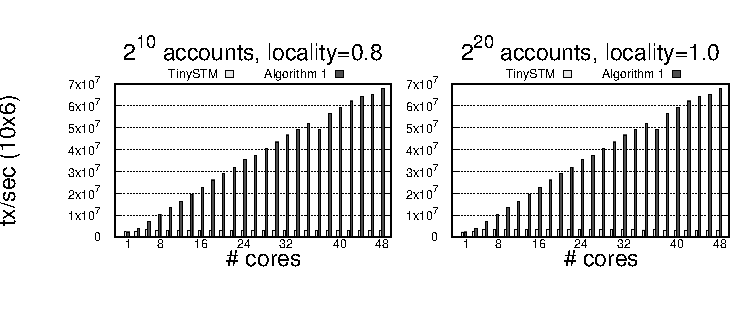
\includegraphics[scale = 1.0]{results/intset/bank.pdf}
	\caption{Bank Benchmark. Left: 80\% locality. Right: 100\% locality.\label{fig:benchmarking:bank}}
\end{figure}

\begin{figure}[!t]
	\centering
	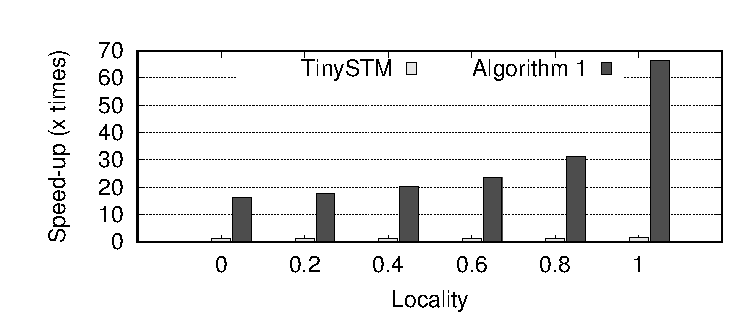
\includegraphics[scale = 0.8]{results/bank-speedup/bank-speedup.pdf}
	\caption{Bank Benchmark. Speed-up of our algorithm for different locality levels. In this experiment, we always use 48 cores.\label{fig:benchmarking:bank:speedup}}
\end{figure}


\subsection{Benchmark: Linked-list}

The linked-list benchmark consists in modifying a sorted linked list concurrently. 
Each thread randomly adds or removes a node from the list. 
We run this benchmark with a range of 512 (meaning that each thread randomly adds/removes a value comprised between -255 and +256) and a linked list initialized with 256 values.
Figure~\ref{fig:benchmarking:llrb}(left) reports our results.

The results show that the global clock outperforms our implementation. 
This is due to the high contention in this application that causes our optimistic algorithm to abort \ft{that's not the right verb} many transactions.

\begin{figure}[!t]
	\centering
	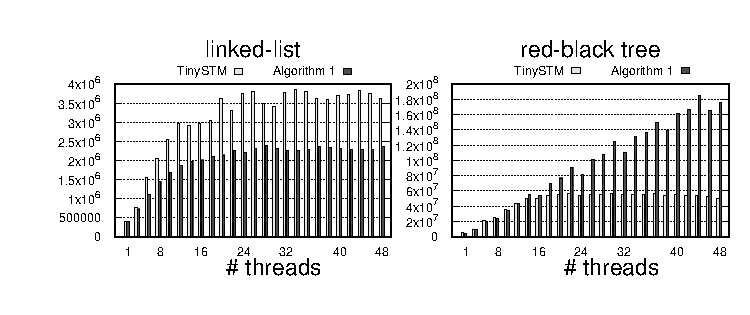
\includegraphics[scale = 1.0]{results/intset/ll-rb.pdf}
	\caption{Linked-list (left) and Red-Black tree (right) benchmarks. Y-axis: transactions/sec. \label{fig:benchmarking:llrb}}
\end{figure}

\subsection{Reb-black tree}

The red-black tree benchmark is similar to the linked-list benchmark except that the values are stored in a self-balancing binary search tree. 
We run this benchmark with a range of $10^7$ values, and a binary tree initialized with $10^5$ values.
Figure~\ref{fig:benchmarking:llrb}(right) reports our results.

When using the global clock, the performance of this application improves linearly up to 12 threads. 
It then stalls to approximately 50 millions transactions per second.

On this application, our implementation scales linearly as the number of threads grows. 
It achieves 176 millions transactions per second with 48 threads.
%
In this benchmark, the likelyhood of a concurrent transaction is very low because of the high number of values in the tree. However,\ft{explain why the global clock performs poorly}.
%

\section{Related Work}
\labsection{relatedwork}

Software transactional memory systems must handle a tradeoff between consistency and performance.
It is however impractical to take into account all possible combinations of read and write conflicts, as it would lead to leargely inefficient solutions. 
%A conflict detection, taking into account all possible combinations of read and write conflicts would just not be efficient. 
Therefore, several mechanisms were introduced to reduce the effort of conflict detection and increase concurrency. 
DSTM~\cite{herlihy2003software} validates all previously accessed object when a new object is about to be opened. 
However, this approach does not scale, and its complexity is quadratic to the number of opened objects within a transaction.

Several time-based STM designs use a global version clock (e.g., Riegel \cite{riegel2006lazy}) to avoid the effort of incrementally validating the read set at commit time. 
TinySTM~\cite{FelberFMR10} is a time-based STM that uses a lazy snapshot technique. 
On commit the TM assigns a timestamp from the global clock to the currently written objects. 
Any transaction constructs a snapshot of linearization points for ensuring consistency. 
By keeping a validity interval of timestamps, it can be verified whether a validation is really necessary. 
We use TinySTM as baseline for our evaluation.

The authors of \cite{zhang2008commit} compare Transactional Locking II (TL2)~\cite{dice2006transactional}, Lazy Snapshot (LSS)\cite{riegel2006lazy} and Global Commit Counter (GCC)~\cite{spear2006conflict}. 
All of them require a new timestamp for each update transaction (total order).
Their approach perform unnecessary updates on the global counter thus leading to unnecessary validations. 
The authors provide several commit alternatives to solve these issues and reducing further unnecessary validations.

New challenges arise when considering multicore architectures and cache coherency strategies for NUMA architectures. 
Clock contention~\cite{6121290} is one of the major issues. 
In a multi-core system with several processors and separate caches, cache coherence messages are required on each update of the clock, which happens frequently. 
Transaction throughput is therefore limited.

To tackle these issues the authors of \cite{Avni:2008} introduce TL2C, which consider a distributed counter --- one per thread. 
The clock values propagate to a \emph{dlock} table with $n-1$ lock entries of different threads. 
During a validation phase, this cache is used, which may however lead to unnecessary aborts. 
Another issue is that the storage of the timestamps might not scale with the number of threads.

In \cite{6121290} the authors adapt TL2 to TrC-MC~\cite{chan2011trc} (transactional consistency for multicore), which groups threads into so-called \textit{zones}. 
Zones share a clock and a clock table.\vs{add a sentence to explain why this is relevant} 
To avoid unnecessary aborts, TrC-MC adopts a timestamp extension mechanism.
TrC-MC compares favourably against TL2 in terms of aborted transsactions.  
%Still the number of aborts are increased, while lower than caused by TL2C.

\vs{add ProteusTM~\cite{didona2016proteustm}}
\vs{add PODC'10 NUMA-aware TM ~\cite{Lu:2010:BAN:1835698.1835713}}
\vs{add ~\cite{Mohamedin:2016:DNC:2851141.2851189}}

\vs{Complete section with 2/3 sentences about how why NumaSTM is different }
\vs{cite ~\cite{nguyen2017scalable}}
%%Why is distributed TM not a relevant work
%%get some more from 612...
%%TODO, why is ours better?

% RWCounter (Lev & Moir) 
% this solution is still global 

% Maintaining Consistent Transactional States without a Global Clock, Avni & Shavit
% space suage: O(m) per thread.
% each transaction got a vector clock inddicating the ts at which other transactions started
% each location got a timestamp pair (x.ts,x.owner), where x.owner is the thread that wrote x last.
% upon reading x, T compare x.ts to  its ts and abort if x.ts[x.owner] > T.ts[x.owner]
% no forward reading possible, thus more false abprt:
%
% This algorithm is SSER but has two main disadvantages
% 1) 
% ``We argue that a TLC transaction will always fail if it attempts 
% to read a location that was written by some other transaction after it started.''
% example of spurious abort: w_p(x).c_p.r_q(x).w_q(y).c_p.r_{q'}(y).a_{q'}.r_{q'}(x).a_{q'}
% the progress property of this STM is very weak, namely
% if the transaction starts from a quescient state and it repeatdly executed and there is no concurrent transaction, then it commits.
% 2) abortion due to non-causally consistent snapshot
% our appraoch does not have this problem


%% With multiple CPUs, each with its own clock, its impossible to guarantee that the crystals
%% don’t differ after some amount of time even when initially set accurately. In practice, all clocks
%% counters will run at slightly different rates. This clock skew brings several problems that can occur
%% and several solutions as well, some more appropriate than others in certain contexts.
%% The Time Stamp Counter was once an excellent high-resolution, low-overhead way for a program to get CPU timing information. With the advent of multi-core/hyper-threaded CPUs, systems with multiple CPUs, and hibernating operating systems, the TSC cannot be relied upon to provide accurate results — unless great care is taken to correct the possible flaws: rate of tick and whether all cores (processors) have identical values in their time-keeping registers. There is no promise that the timestamp counters of multiple CPUs on a single motherboard will be synchronize
%% Relying on the TSC also reduces portability, as other processors may not have a similar feature

%% Thanks for all the inputs: Here's the conclusion for this discussion: The TSCs are synchronized at the initialization using a RESET that happens across the cores and processors in a multi processor/multi core system. And after that every Core is on their own. The TSCs are kept invariant with a Phase Locked Loop that would normalize the frequency variations and thus the clock variations within a given Core and that is how the TSC remain in sync across cores and processors.

%% https://stackoverflow.com/questions/10921210/cpu-tsc-fetch-operation-especially-in-multicore-multi-processor-environment
%% https://github.com/dterei/tsc

%% PCL theorem

% the alg. of shvit et al. exhibits a very weak progress property, namely if the transaction is retried infinitely often it eventually commits.

%%   Computer designs that exploit data locality with multiple cache levels, such as non-uniform memory architectures (NUMA), have to reduce the amount of global operations to improve application performance or take special care to address traffic congestions\cite{dashti2013traffic}.


\section{Conclusion}
\labsection{conclusion}

Transactional memory systems must handle a tradeoff between consistency and performance.
It is impractical to take into account all possible combinations of read and write conflicts, as it would lead to largely inefficient solutions.
%% For instance, accepting $\RCAD$ histories brings only a small performance benefits in the general case~\cite{hans16}.

%Inspired by line of research, 
This paper introduces a new consistency criterion, named stricter serializability ($\SPSER$).
Workloads executed under $\SPSER$ are opaque when the object graph forms a tree and transactions traverse it top-down.
We present an algorithm to attain this criterion together with a proof of its correctness.
Our evaluation based on a fully implemented prototype demonstrates that such an approach is very efficient in weakly-contended workloads.

% move from SSER to SSER+ (i.e., alg. transform) ?



{
  \footnotesize
  \bibliographystyle{abbrvnat}
  \bibliography{bib/nicolas,bib/psutra,bib/mshapiro,bib/paper}
}  

\end{document}
